\documentclass[aps,prl,twocolumn,groupedaddress]{revtex4-1}
% \documentclass[aps,twocolumn,secnumarabic,balancelastpage,amsmath,amssymb,nofootinbib]{revtex4-1}
\usepackage{amsmath}
\usepackage{amssymb}
\usepackage{amsfonts}
\usepackage{color}
\usepackage{graphics}
\usepackage[pdftex]{graphicx}
\usepackage[utf8x]{inputenc}
\usepackage[colorlinks=true]{hyperref}

\usepackage[final]{fixme}
\fxsetup{layout=inline}

\newcommand{\ud}{\mathrm{d}}
\newcommand{\ue}{\mathrm{e}}
\newcommand{\ui}{\mathrm{i}}
\newcommand{\res}{\mathrm{Res}}
\newcommand{\Tr}{\mathrm{Tr}}
\newcommand{\dsum}{\displaystyle\sum}
\newcommand{\dprod}{\displaystyle\prod}
\newcommand{\dlim}{\displaystyle\lim}
\newcommand{\dint}{\displaystyle\int}
\newcommand{\fsno}[1]{{\!\not\!{#1}}}
\newcommand{\texp}[2]{\ensuremath{{#1}\times10^{#2}}}
\newcommand{\dexp}[2]{\ensuremath{{#1}\cdot10^{#2}}}
\newcommand{\eval}[2]{{\left.{#1}\right|_{#2}}}
\newcommand{\paren}[1]{{\left({#1}\right)}}
\newcommand{\lparen}[1]{{\left({#1}\right.}}
\newcommand{\rparen}[1]{{\left.{#1}\right)}}
\newcommand{\abs}[1]{{\left|{#1}\right|}}
\newcommand{\sqr}[1]{{\left[{#1}\right]}}
\newcommand{\crly}[1]{{\left\{{#1}\right\}}}
\newcommand{\angl}[1]{{\left\langle{#1}\right\rangle}}
\newcommand{\tpdiff}[4][{}]{{\paren{\frac{\partial^{#1} {#2}}{\partial {#3}{}^{#1}}}_{#4}}}
\newcommand{\tpsdiff}[4][{}]{{\paren{\frac{\partial^{#1}}{\partial {#3}{}^{#1}}{#2}}_{#4}}}
\newcommand{\pdiff}[3][{}]{{\frac{\partial^{#1} {#2}}{\partial {#3}{}^{#1}}}}
\newcommand{\diff}[3][{}]{{\frac{\ud^{#1} {#2}}{\ud {#3}{}^{#1}}}}
\newcommand{\psdiff}[3][{}]{{\frac{\partial^{#1}}{\partial {#3}{}^{#1}} {#2}}}
\newcommand{\sdiff}[3][{}]{{\frac{\ud^{#1}}{\ud {#3}{}^{#1}} {#2}}}
\newcommand{\tpddiff}[4][{}]{{\left(\dfrac{\partial^{#1} {#2}}{\partial {#3}{}^{#1}}\right)_{#4}}}
\newcommand{\tpsddiff}[4][{}]{{\paren{\dfrac{\partial^{#1}}{\partial {#3}{}^{#1}}{#2}}_{#4}}}
\newcommand{\pddiff}[3][{}]{{\dfrac{\partial^{#1} {#2}}{\partial {#3}{}^{#1}}}}
\newcommand{\ddiff}[3][{}]{{\dfrac{\ud^{#1} {#2}}{\ud {#3}{}^{#1}}}}
\newcommand{\psddiff}[3][{}]{{\frac{\partial^{#1}}{\partial{}^{#1} {#3}} {#2}}}
\newcommand{\sddiff}[3][{}]{{\frac{\ud^{#1}}{\ud {#3}{}^{#1}} {#2}}}
\newcommand{\eff}{ef\! f}
%Nick redefined fxnote so that the notes could be seen in the PDF since that is what Kang-Kuen is editing
\renewcommand{\fxnote}[1]{{\textbf{[#1]}}}

\begin{document}
\title{Motional Quantum Ground-State Cooling Outside the Lamb-Dicke Regime}
\author{Yichao Yu}
\author{Nicholas R. Hutzler}
\author{Jessie T. Zhang}
\author{Lee R. Liu}
\author{Kang-Kuen Ni}
\email{ni@chemistry.harvard.edu}
\affiliation{Department of Chemistry and Chemical Biology, Harvard University, Cambridge, Massachusetts, 02138, USA}
\affiliation{Department of Physics, Harvard University, Cambridge, Massachusetts, 02138, USA}
\affiliation{Harvard-MIT Center for Ultracold Atoms, Cambridge, Massachusetts, 02138, USA}

\date{\today}

\begin{abstract}
  Single neutral atoms trapped in optical tweezers are a promising system for many applications
  in quantum information and simulation.
  These applications typically require complete quantum control, including motional states, which requires cooling of the trapped atoms.
  We report Raman sideband cooling of a single sodium atom to its three-dimensional
  motional ground state in an optical tweezer.
  Despite having a very large Lamb-Dicke parameter, high initial temperature and
  large differential AC Stark shift in the excited state,
  we achieve a ground state preparation fidelity of $77(4)\%$ after a few hundred ms of cooling
  by using novel cooling techniques such as addressing high order Raman sidebands.
  We demonstrate that Raman sideband cooling to the 3D motional ground state is applicable outside the Lamb-Dicke regime, for example in
  systems where tight confinement and low initial temperature are difficult to realize.
  The is particularly relevant for systems which are challenging to laser-cool,
  such as molecules and exotic atoms, and opens up a new approach for further cooling
  of these systems.
\end{abstract}

\maketitle

\begin{figure*}
  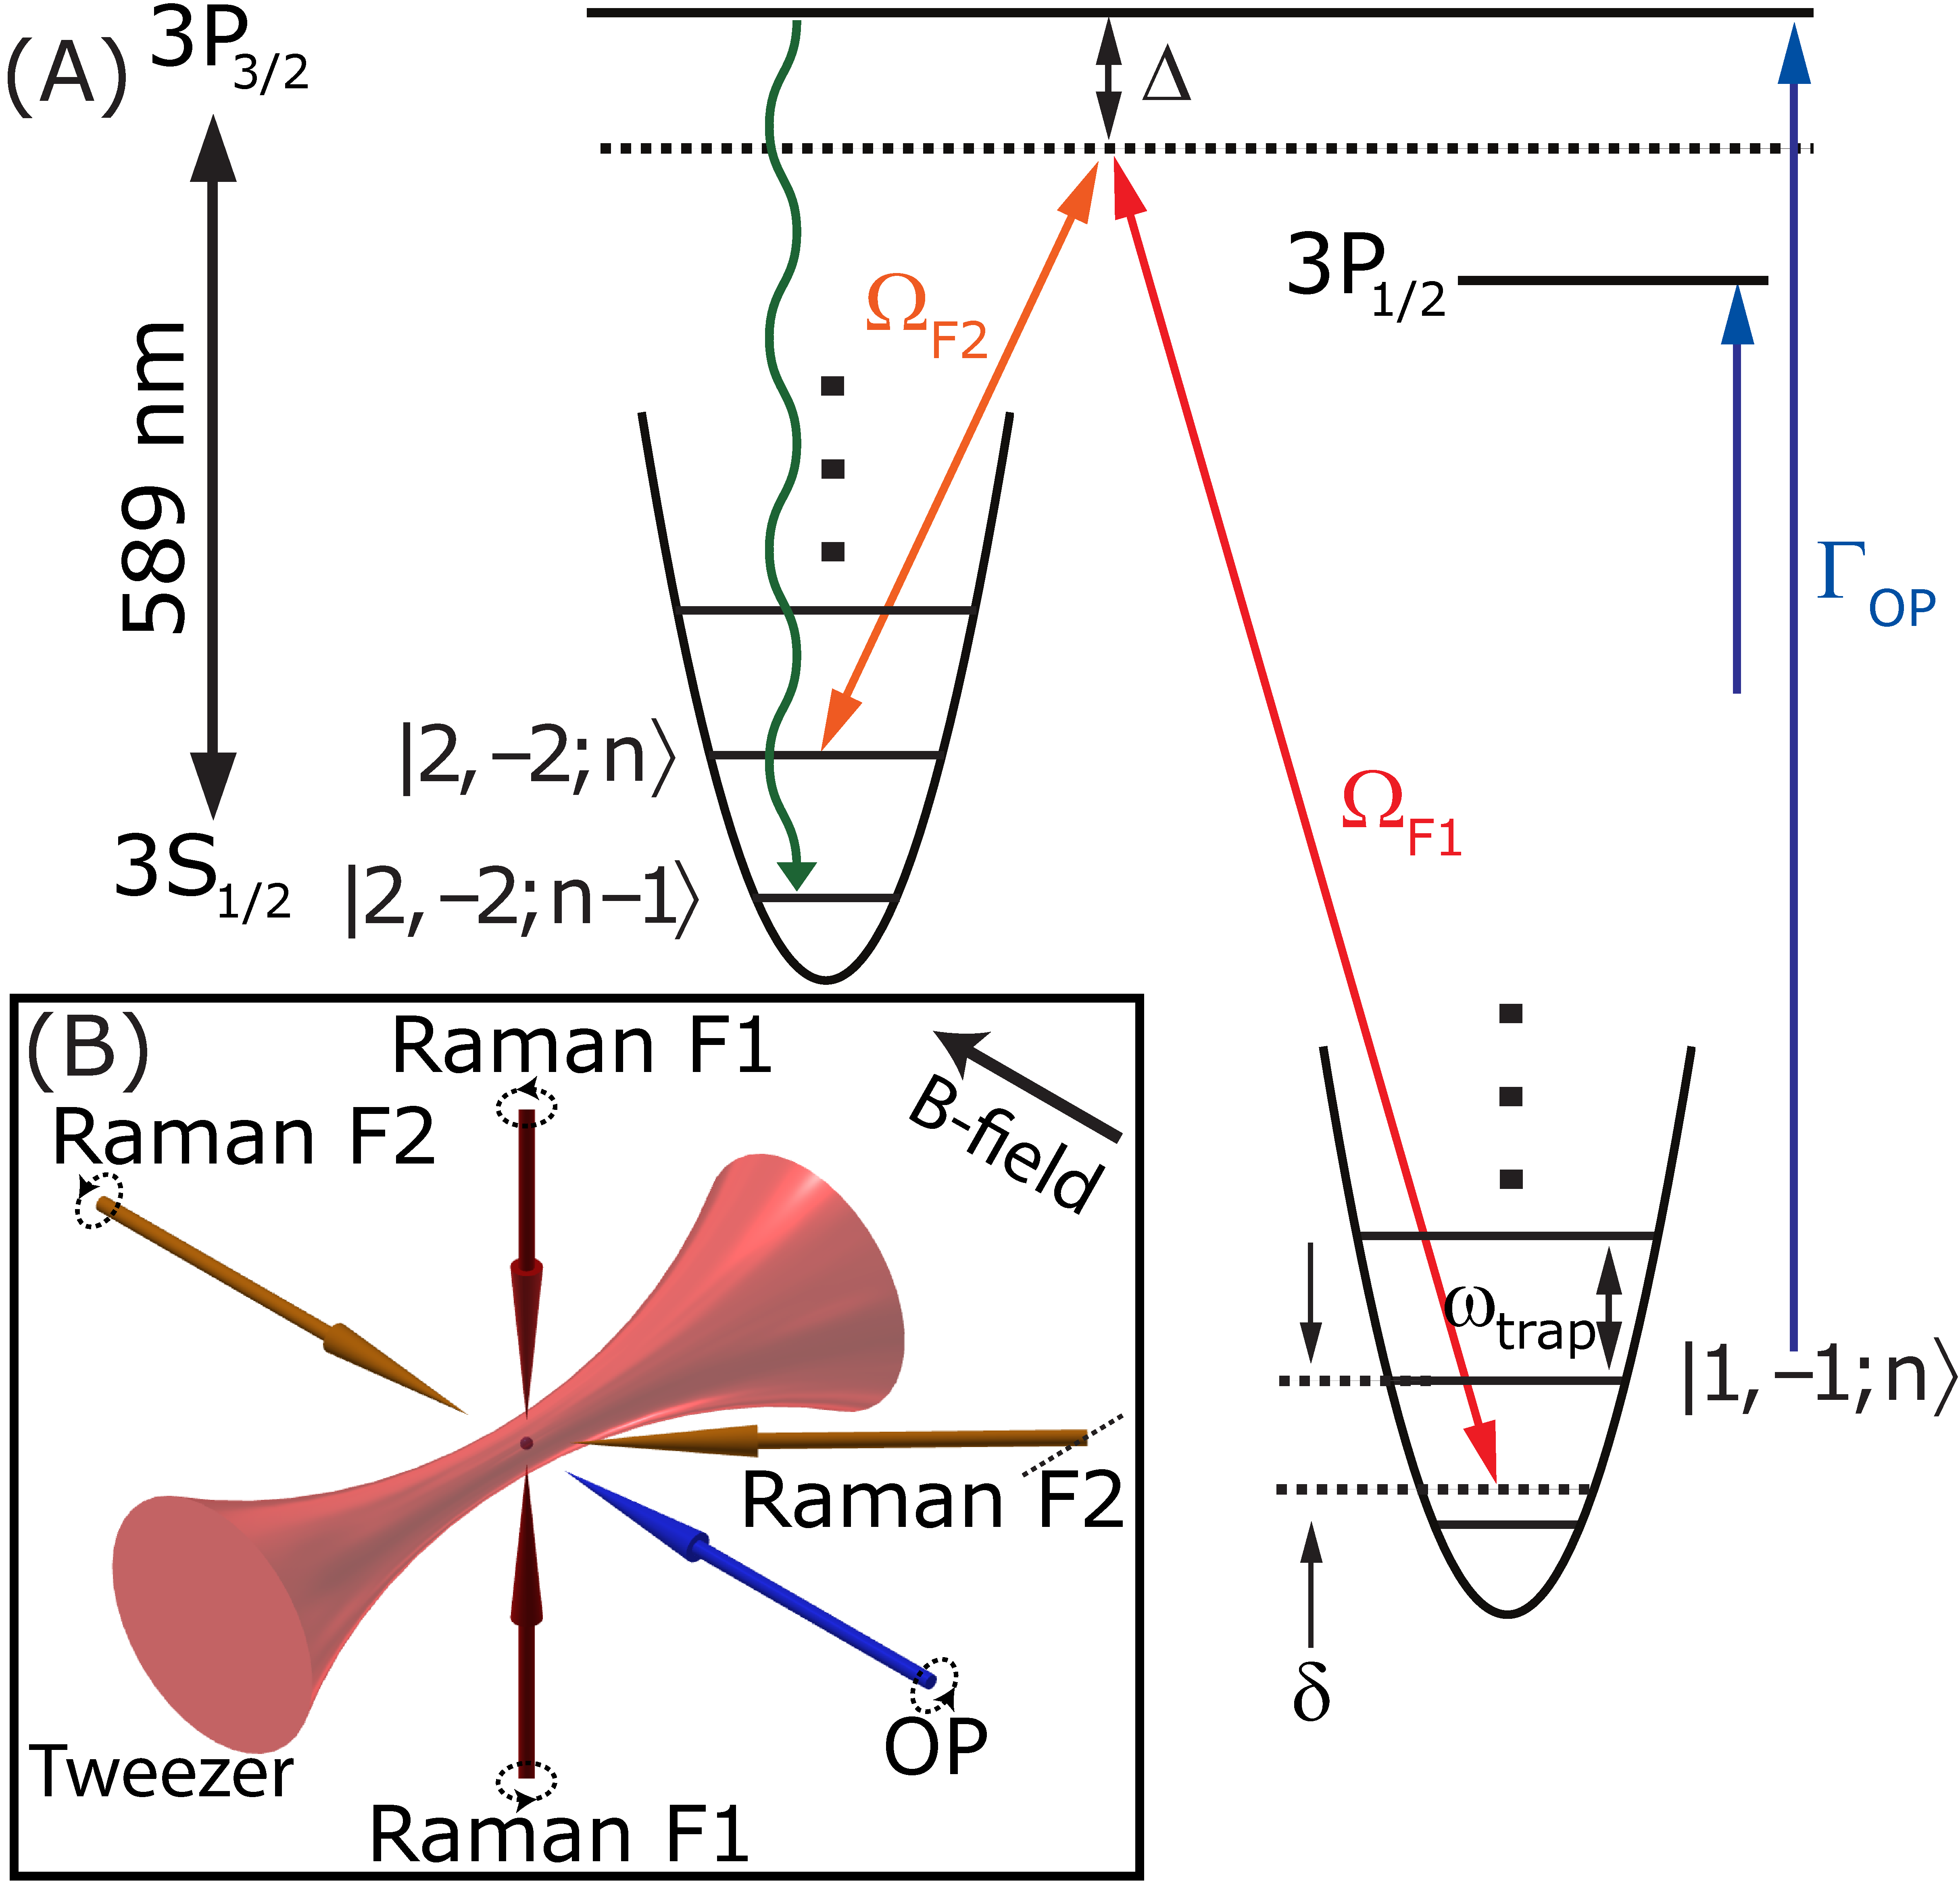
\includegraphics[height=5.2cm]{imgs/Na_RSC_schematic.pdf}
  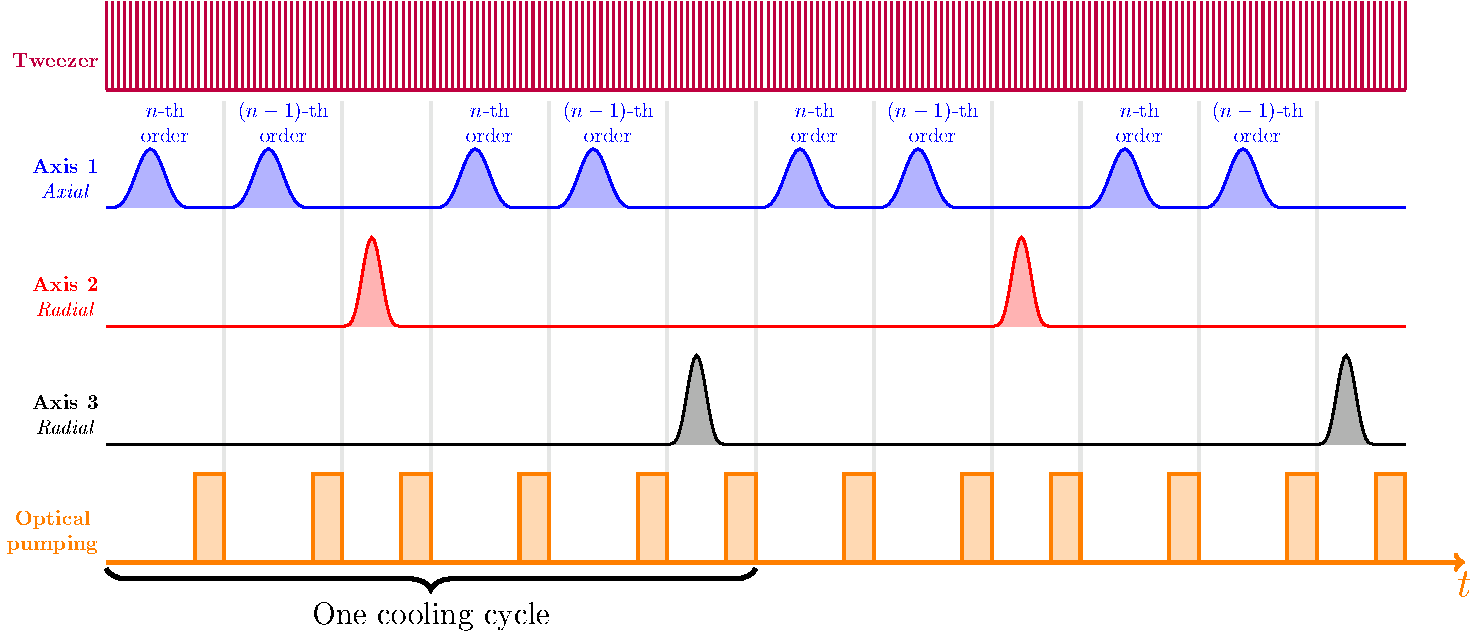
\includegraphics[height=4.5cm]{sequence.pdf}
  \caption{(A) Energy levels and schematic of Raman sideband cooling.
    The Raman transitions have a one photon detuning $\Delta=25$ GHz from the D2 line.
    We use D1 light with $\sigma^-$ polarization to repump atoms out of $|F=2,m_F=-1\rangle$
    state to minimize heating on the atom in $|F=2,m_F=-2\rangle$ state
    (B) Geometry and polarizations of the Raman and optical pumping beams relative to the
    optical tweezer and bias magnetic field.
    (C) Schematic of the cooling sequence. The tweezer switches at 3 MHz to
    reduce light shifts during optical pumping. Each cooling cycle consists of $8$ pulses.
    The four axial pulses are addressing two neighboring cooling orders.
    The two pulses in each radial directions are either addressing two neighboring cooling orders
    or having different length on the first order when most of the population are below $n=3$
    towards then end of the cooling sequence.
    \label{f-setup}}
\end{figure*}
\begin{figure}[b]
  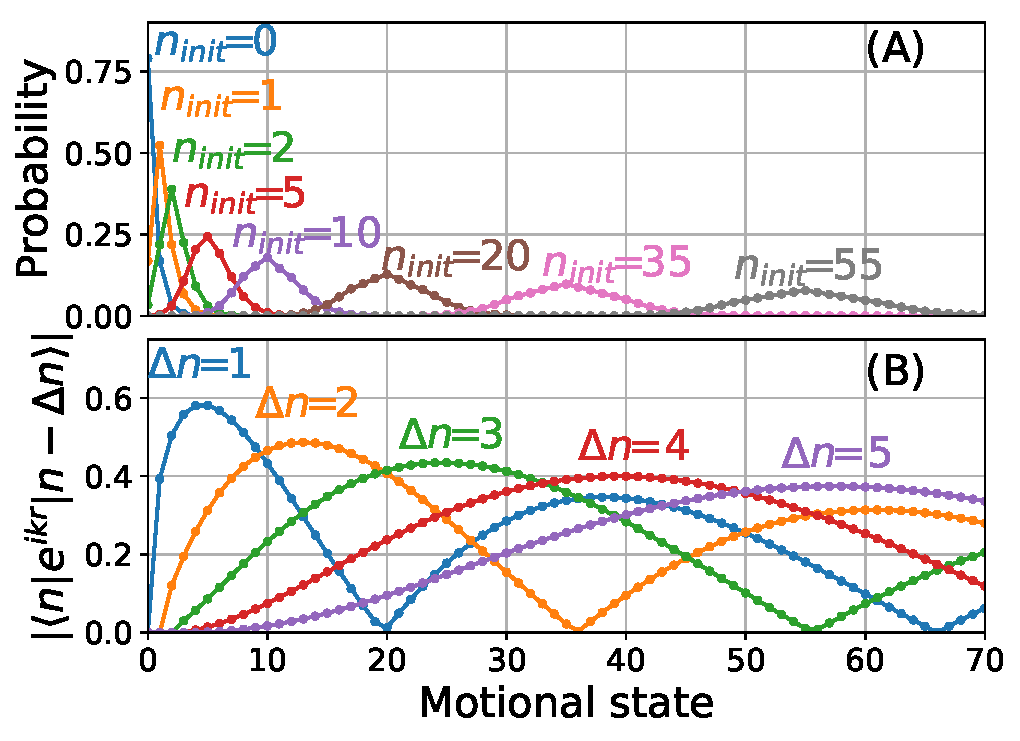
\includegraphics[width=8.5cm]{imgs/fig2_raman_op.pdf}
  \caption{Matrix elements and heating as a function of motional state.
    The range plotted covers $95\%$ of the initial thermal distribution.
    (A) Matrix elements for Raman transition in the axial direction showing deviation from
    $\sqrt{n}$ scaling and multiple minimums for different sideband orders.
    (B) Average change in motional state after the optical pumping step for all three axis.
    Due to the large Lamb-Dicke parameter,
    there is a high probability of $n$ changing especially in the axial direction.
    \label{f-ld}}
\end{figure}
\begin{figure*}
  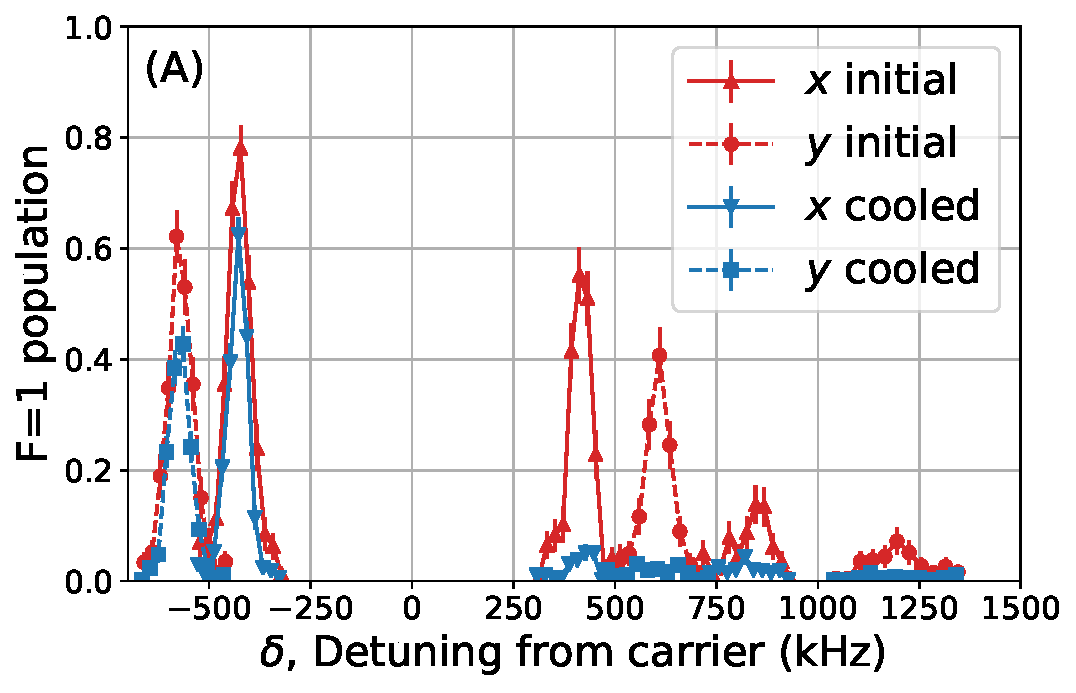
\includegraphics[height=4.2cm]{imgs/spectrum_r.pdf}
  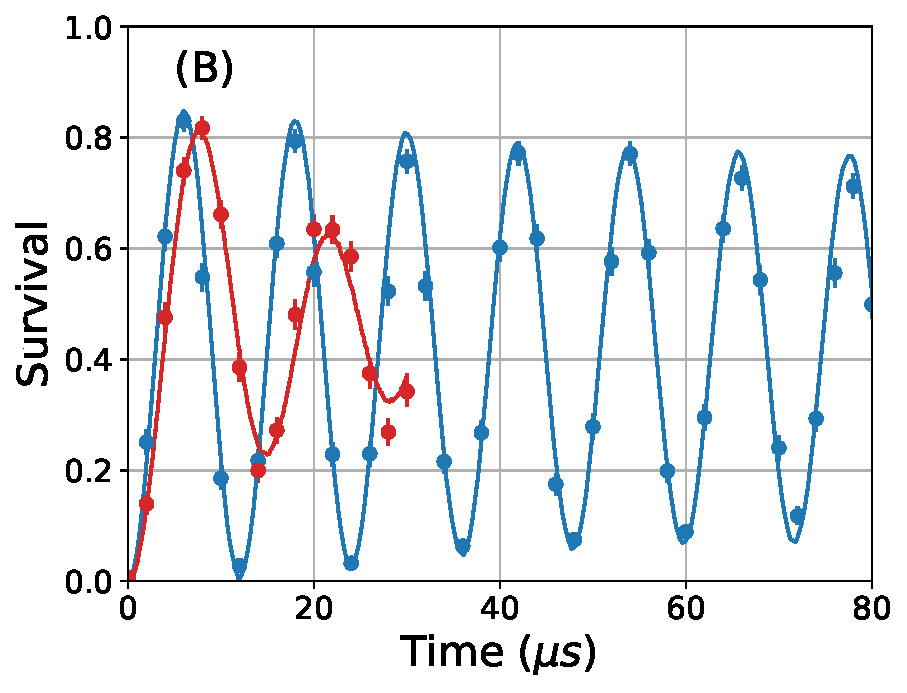
\includegraphics[height=4.2cm]{imgs/rabi_flop_r3_0.pdf}
  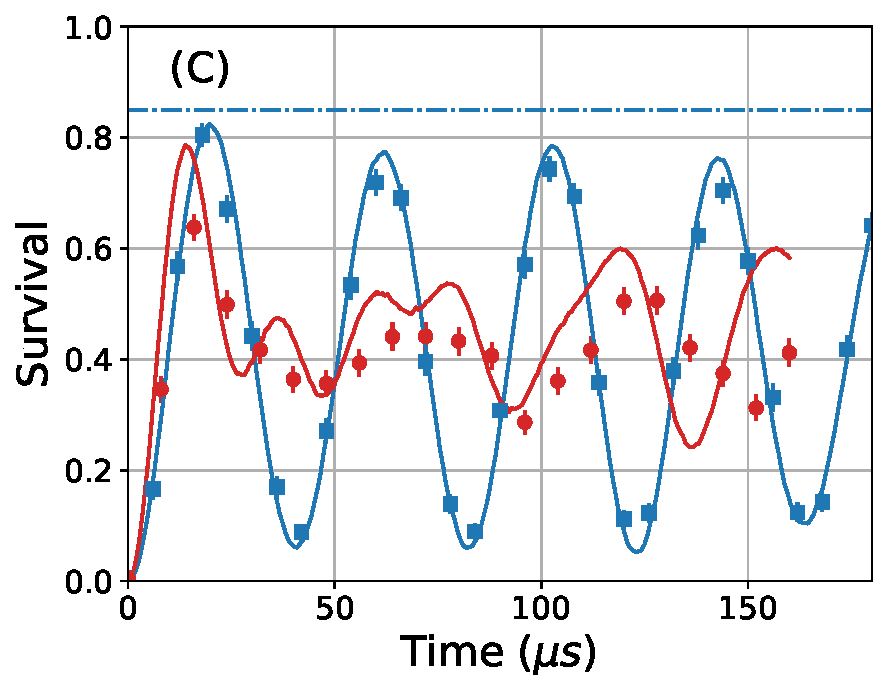
\includegraphics[height=4.2cm]{imgs/rabi_flop_r3_p1.pdf}
  \caption{(A) Radial Raman sideband spectrum of first order heating, first order cooling and
    second order cooling before and after Raman sideband cooling.
    (B,C) Rabi flopping on axis 3 (B) carrier and (C) first order heating sideband
    before (red) and after (blue) cooling.
    Solid lines in (B) and (C) are theoretical calculation of the Rabi flopping.
    The blue lines corresponds to a ground state probability of $93\%$ after cooling and
    the red lines corresponds to a thermal distribution of $70$ $\mu$K before cooling.
    \label{f-radial}}
\end{figure*}
\begin{figure*}
  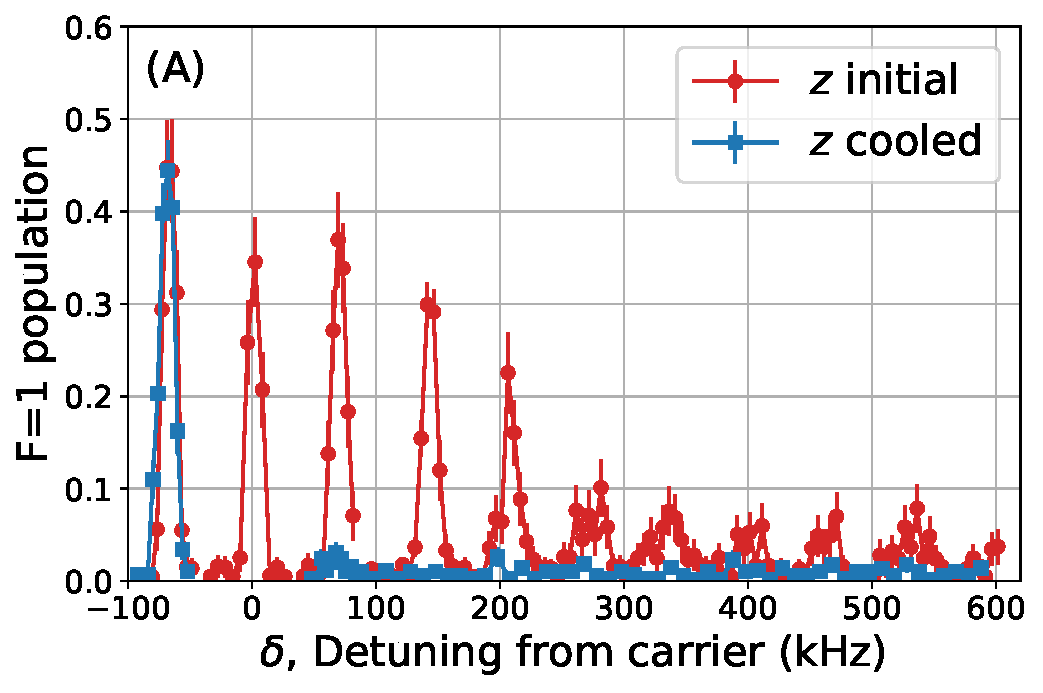
\includegraphics[height=4.2cm]{imgs/spectrum_a1.pdf}
  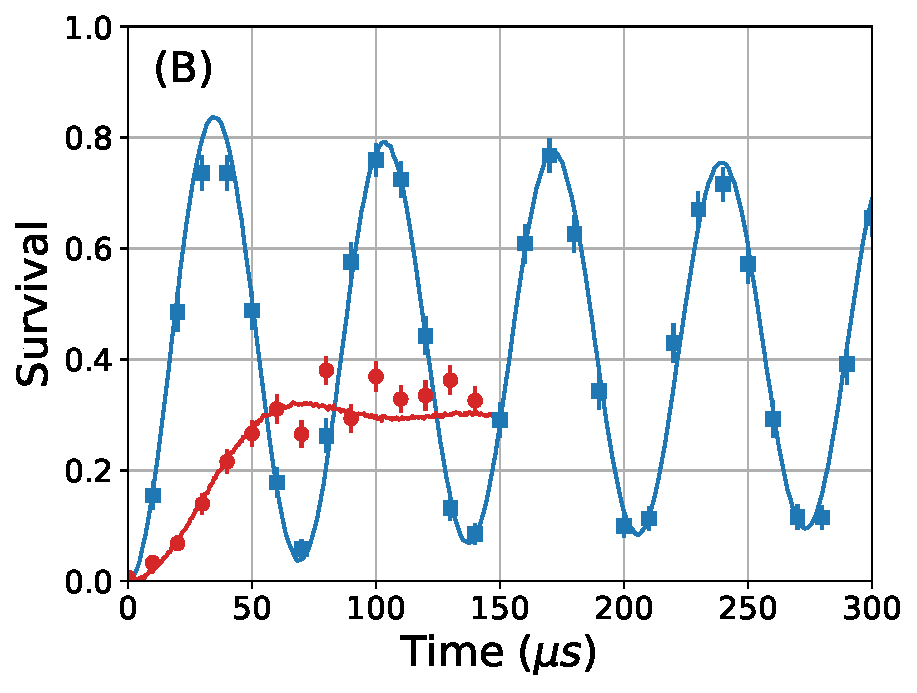
\includegraphics[height=4.2cm]{imgs/rabi_flop_a1_0.pdf}
  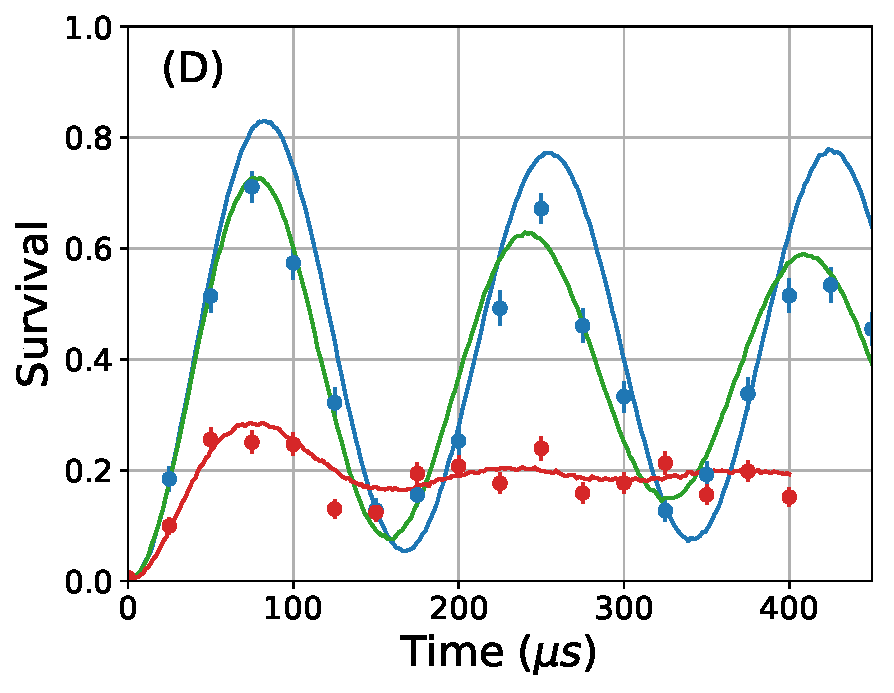
\includegraphics[height=4.2cm]{imgs/rabi_flop_a1_p1.pdf}
  \caption{(A) Axial Raman sideband spectrum from first order heating to eighth order cooling
    before and after Raman sideband cooling.
    The data for the second and higher orders of cooling sidebands are taken with 150 $\mu$s
    pulse time and the rest are taken with 125 $\mu$s pulse time.
    (B,C) Rabi flopping on axial (B) carrier and (C) first order heating sideband
    before (red) and after (blue) cooling.
    Solid lines in (B) and (C) are theoretical calculation of the Rabi flopping.
    The blue and green lines corresponds to a ground state probability of $92\%$ after cooling and
    the red lines corresponds to a thermal distribution of $70$ $\mu$K before cooling.
    The blue lines does not take into account the effect of decoherence due to resonance
    fluctuation. By comparing it to the green line in (C), which includes a $3$ kHz fluctuation,
    we can clearly see that this effect is the strongest for the after cooling data on
    the axial heating sideband where the Rabi frequency is the lowest.
    \label{f-axial}}
\end{figure*}

Systems of individual neutral atoms trapped in optical tweezers are an exciting platform to study
quantum information, quantum chemistry, and quantum simulation of many-body systems\cite{Schlosser2001,DeMille2002,Muller2014Rydberg}.
This approach provides full single-site resolution and control,
and can feature long-range interactions by using Rydberg atoms, polar molecules,
or dipolar atoms\cite{Micheli2006,Muller2014Rydberg,Walker2012}.
Polar molecules in particular offer the additional advantages of long-lived internal states
and a high degree of tunability, including the shape, range,
and strength of the interaction\cite{Sortais2007,Beugnon2007,Ni2009}.
Optical tweezers can also be re-arranged in real-time,
allowing rapid preparation of atoms in complex geometries with high fidelity
\cite{Carpentier2013,Weiss2004}.

In order to achieve long coherence times and full quantum control of the system,
it is typically necessary to cool the atom to the
three dimensional motional ground state in the optical tweezer.
This has been demonstrated for neutral Rb\cite{Thompson2013,Kaufman2012}
and Cs\cite{Li2012,Liu2017}
in experiments that had low initial temperature and small Lamb-Dicke parameter.
These features may not be easily achievable for other systems,
such as directly laser-cooled polar molecules\cite{Shuman2010,Chae2017},
or atoms with challenging sub-Doppler cooling such as Na, K, and Li\cite{Shahriar1993a,Colzi2016,Salomon2013,Salomon2015}.
In this letter, we cool single sodium atoms trapped in optical tweezers to
the motional ground state with Raman sideband cooling.
Despite having a large Lamb-Dicke parameter and high initial temperature,
we are able to achieve a ground state probability of $77(4)\%$
by utilizing several new cooling techniques and a carefully optimized cooling sequence.
Our approach is quite general, and opens up ground-state cooling for other systems.

The Raman sideband cooling we use to achieve the high ground state preparation fidelity
consists of multiple cycles of laser pulses to manipulate the internal and
motional states of the atoms.
Figure \ref{f-setup}A shows the schematic of the energy levels and the cooling sequence
in our setup.
Each cooling cycle starts with the sodium atom in the $|F=2, m_F=-2\rangle$
ground electronic state and a certain vibration state $n$.
In the first step, a Raman pulse drives a transition to the motional state $n-\Delta n$
to reduce the motional energy while also changing the internal state to $|F=1, m_F=-1\rangle$.
In the second step, which finishes the cooling cycle,
an optical pumping pulse bring the atom back to the $|F=2, m_F=-2\rangle$ state to take away
the entropy via the spontaneously emitted photon.
The second step could also change the motional state of the atoms and result in heating.
The possibility for this to happen for an atom in the motional level $n$
is approximately proportional to the effective Lamb-Dicke (LD) parameter
$\eta^{OP}_{\eff}=\sqrt{2n+1}\eta^{OP}$ where $\eta^{OP}=k^{OP}\sqrt{\hbar/2m\omega}$
is the LD parameter for optical pumping (OP), $k^{OP}$ is the wavenumber of the OP light, $m$ is the mass of the atom, and $\hbar$ is the reduced Planck constant.

In order to reduce OP scattering on the $|F=2, m_F=-2\rangle$ state, which would causing heating, we use a $\sigma^-$-polarized laser resonant with the D1 line to address atoms in the $F=2$ state, so that $|F=2, m_F=-2\rangle$ is dark.  Compared to using a D2 OP beam, we find a reduction in the scattering rate of a factor of $130(20)$.


The geometry of the relevant beams and their polarizations is shown in figure \ref{f-setup}B.
The optical tweezer has one weakly confined axial direction (axis $1$) and
two more strongly confined radial directions (axis $2$ and $3$).
Multiple pairs of beams are used to drive the Raman transition during cooling in order to
isolate and maximize the coupling to different trap axis.

In order to perform Raman sideband cooling efficiently and minimize
the heating during the optical pumping, we need to have a low initial temperature and
a small LD parameter. However, since the LD parameter $\eta\propto 1/(\sqrt[4]{m}\lambda)$ where $m$ is the mass of the atom and $\lambda$
is the wavelength of the atomic transition,
it is larger for sodium at a given trap depth due to its low mass and short D line wavelength.
With 45 mW of power in the trap, we measure trapping frequencies of
$\{\omega_1,\omega_2,\omega_3\}/2\pi = \{69(1), 430(4), 590(5)\}\ \text{\text{kHz}}$
which corresponds to optical pumping LD parameters of
$\{\eta^{OP}_1,\eta^{OP}_2,\eta^{OP}_3\} = \{0.602(5), 0.241(2), 0.206(1)\}$
Moreover, due to the small hyperfine splitting in the $3^2P_{3/2}$ manifold,
the sub-Doppler cooling in sodium is also less efficient and we start the
Raman sideband cooling with a initial temperature of 70 $\mu$K. Combined with the high $\eta$, this gives us a initial effective optical pumping LD parameters of
$\{\eta^{OP}_{1\eff},\eta^{OP}_{2\eff},\eta^{OP}_{3\eff}\} = \{4.0(1), 0.67(2), 0.50(1)\}$
As a result, there is a very high average change of motional state during the optical pumping step
(figure \ref{f-ld}B). The averaged change in motional states over the initial distribution
is $2.4$ in the axial direction.
Compare to $0.89-0.95$ in the axis with the weakest confinement in previous experiments
\cite{Thompson2013,Kaufman2012,Li2012,Liu2017} this causes greater uncertainty in the motional
state making it harder to cool.

Fortunately, the high LD parameters also
provide us with tools to overcome this issue. The Raman transitions in our configuration have $\{\eta^R_{1},\eta^R_{2},\eta^R_{3}\} = \{0.40(1), 0.341(2), 0.291(1)\}$. As shown in
figure \ref{f-ld}A, this results in strong coupling to higher orders
of cooling sidebands, especially for high motional states.
This enables cooling of atoms in high motional states by driving higher order Raman sidebands,
removing more motional energy in a single cooling pulse and offsetting the effect of heating. Since the heating probability is higher for high motional states,
cooling on these high order sidebands can greatly suppress the high heating during
optical pumping during the initial cooling. Since the coupling strength of different orders
do not reach their minimums at the same time, using multiple orders of motional sidebands
for cooling also avoids accumulation of population near the coupling minimum of a particular
order, which improves the overall efficiency of the cooling process.

The high initial temperature also causes additional complications beyond large $\eta$.
First, population in high motional states means that the atoms sample
the anharmonicity of the trap away from the harmonic center.
This effect broadens the sidebands and reduces their strengths on resonance,
and therefore the efficiency of cooling, when driven with a single frequency.
In order to overcome this issue, we power broaden the sidebands by increasing the Rabi frequency
so that it is larger than the expected sideband frequencies distribution
which causes all the states to be driven equally.
This limits the Rabi frequency of the Raman pulse on the radial sidebands to be no lower
than tens of kHz.
Second, the deep trap that is needed to trap and image single sodium atom also creates
a very large AC Stark shift in the excited state (as large as 300 MHz).
This creates large, position-dependent detuning for the optical pumping light and mixes the excited state state hyperfine levels,
which affects the branching ratios and increases the number of photons needed for optical pumping.
We solve this issue by switching the trapping light at 3 MHz
during the whole cooling sequence, similar to our loading and imaging process
\cite{Hutzler2017-LightShifts}, but leaving on the OP light with constant intensity.
Due to the large light shift, the OP light is effectively off when the trap light is on.
Since the atom can only be addressed by the optical pumping light when the trap light is off,
the effect of light shift on optical pumping fidelity is suppressed.

Taking all these features into account, we use a Monte-Carlo simulation to verify
the validity of our method.
In the simulation, we can observe the high heating rate due to the high LD parameters
and confirm that by using high order Raman sideband transition in the cooling sequence we can
suppress this effect and reduces the motional energy of the atom faster.
The simulation is also used to guide the optimization of the cooling sequence by exploring the
large parameter space and finding a robust cooling strategy.
As shown in figure \ref{f-setup}C, we found that instead of cooling on only one sideband order
at a time, it is generally more efficient to alternate the cooling pulse between two
neighboring orders (axial) to minimize the accumulation of atom in a state
not addressed by a particular order.
The simulation also shows that an efficient way of cooling on a high order sideband is
to set the Rabi frequency of the Raman transition to perform a $\pi$ pulse for the maximum matrix element of that order over all states (i.e. the maxima in \ref{f-ld}A).
This makes sure we are using each order to cool a range of states that has the strongest
coupling to this order and let other sidebands to cool other states.

The efficiency of this approach diminishes during the last stages of cooling as the atom approaches the ground state.  We therefore finish the sequence by cooling only on the first order sideband while maintaining the alternating order between different axes.
Guided by the simulation results, we construct our initial cooling sequence by first starting
at the highest two observed cooling sideband and decrease the order after cooling on them
for 6 to 15 cycles with the optimum pulse lengths.
This sequence gives good cooling performance which is then experimentally further optimized
by fine tuning of different parameters.

For the more tightly confined radial directions,
we begin the cooling with $\{\bar n_2, \bar n_3\}=3.4(2), 2.5(2)$.
The radial sideband spectra of the initial distribution is shown in figure \ref{f-radial}A
as orange and red lines, where we can clearly see the first order heating,
first order cooling and second order cooling sidebands.
After applying around 1000 cooling pulses cooling in all three dimensions
starting with cooling on the radial second order,
the Raman spectrum with the same parameters is shown in figure \ref{f-radial}A as
blue and green lines, where the first and second order cooling sidebands
on both axis are suppressed.
Given the absence of the second order cooling sideband,
we can estimate the ground state probability in each direction based on the height of
the first order cooling and heating sideband to be $90(2)\%$ and $94(3)\%$.

It is important to note that the large Raman LD parameters $\eta^R$ mean that
we must use caution when measuring the temperature.
Traditional sideband thermometry uses
the ratio of the cooling and heating sidebands to measure $\bar n / (\bar n + 1)$, which relies
on the coupling strength to be proportional to $\sqrt{n}$. However, outside the
LD regime, the coupling strength deviates from this simple scaling rule rapidly as
shown in figure \ref{f-ld}A.
When the atom temperature is still high,
we measure the heights of multiple sidebands to make sure no population is hidden at the
minimum of one sideband order. Once the atom is cooled down, we estimate the temperature
and ground state population under the assumption that only a few states are populated.
We can verify the result via an independent measurement of Rabi flopping on the carrier and
heating sidebands\cite{Meekhof1996}. This data is shown before and after cooling in Figures
\ref{f-radial}B and \ref{f-radial}C.
The data is fitted using same Monte-Carlo simulation we used to simulate the cooling
which yields $89(2)\%$ and $92(2)\%$ showing good agreement between the two methods.

The axial direction is much less confined and therefore has a much higher initial
$\bar n_1=21(2)$ and effective LD parameter of $\eta^{OP}_{eff1}\approx 4.0(2)$,
and is therefore more difficult to cool.
The red line in figure \ref{f-axial}A shows the Raman spectrum in the axial direction
before applying Raman sideband cooling; the clearly resolved sidebands
up to eighth order indicates population in highly-excited motional levels.
Therefore, we begin our cooling sequence by driving Raman transitions on the eighth order axial
cooling sideband. After applying the cooling sequence identical to the one we use to cool
the radial directions, the spectrum is shown in figure \ref{f-axial}A as the blue line.
All of the high order ($\geqslant2$) axial cooling sidebands disappear, and the first order
cooling sideband is strongly suppressed.
The ground state probability calculated from this spectrum is $92(3)\%$.
We can again use Rabi flopping on the carrier and heating sideband to verify this result
similar to the radial direction. In this case, we see very good agreement on the carrier
(figure \ref{f-axial}B) but there is additional decoherence on the axial first order
heating sideband (figure \ref{f-axial}C).
We believe this decoherence is caused by technical noise, which is the most pronounced
on this transition due to its slow Rabi frequency.
The decoherence time scale is consistent with magnetic field fluctuations of $1.5$ mG that we have measured in the lab, which produces
a Zeeman shift of around $3$ kHz.

Combining the axial and radial cooling results,
we have achieved a 3D ground state probability of $77(4)\%$.
We believe this is currently limited by off-resonant scattering from the Raman beams,
which are measured to be between $3$ to $15$ kHz for the detuning and power we use,
and the resonance shift caused by magnetic field fluctuations.
Other imperfections of the current experiement include a $5\%$ loss during the single atom
imaging and an additional $10\%$ due to the heating from the Raman beams during cooling.
We are planing to improve these by increasing the detuning of the Raman beams,
implementing better control of the magnetic field and optimize the temperature during imaging.
We expect these changes to improve the cooling performance even further.
We have shown that despite the difficulty in cooling sodium atoms,
it is possible to achieve reliable three dimensional cooling with significant ground state
probability using new cooling techniques and a optimized cooling sequence.
This opens up the possibility of cooling a large variety of systems to their motional ground
state using Raman sideband cooling that is challenging to laser cool
including molecules and exotic atoms.

% Missing:
% ?? Blackman pulse vs square pulse
% ?? Start from highest visible order
% In the text, more description
% Detail in appendix

\bibliography{paper}
\end{document}
